\documentclass[../Dokumentacja.tex]{subfiles}
\begin{document}
\subsection{Game Master}
Moduł Game Master przeprowadza całą rozgrywkę w The Project Game. Przechowuje aktualny stan gry,
a każda akcja Agentów musi najpierw zostać odnotowana i zwalidowana przez niego.
Cała komunikacja między Agentami i Game Masterem odbywa się poprzez moduł Serwera Komunikacyjnego.
Game Master odpowiada także za dostarczenie interfejsu graficznego do prezentacji stanu gry i wyników.

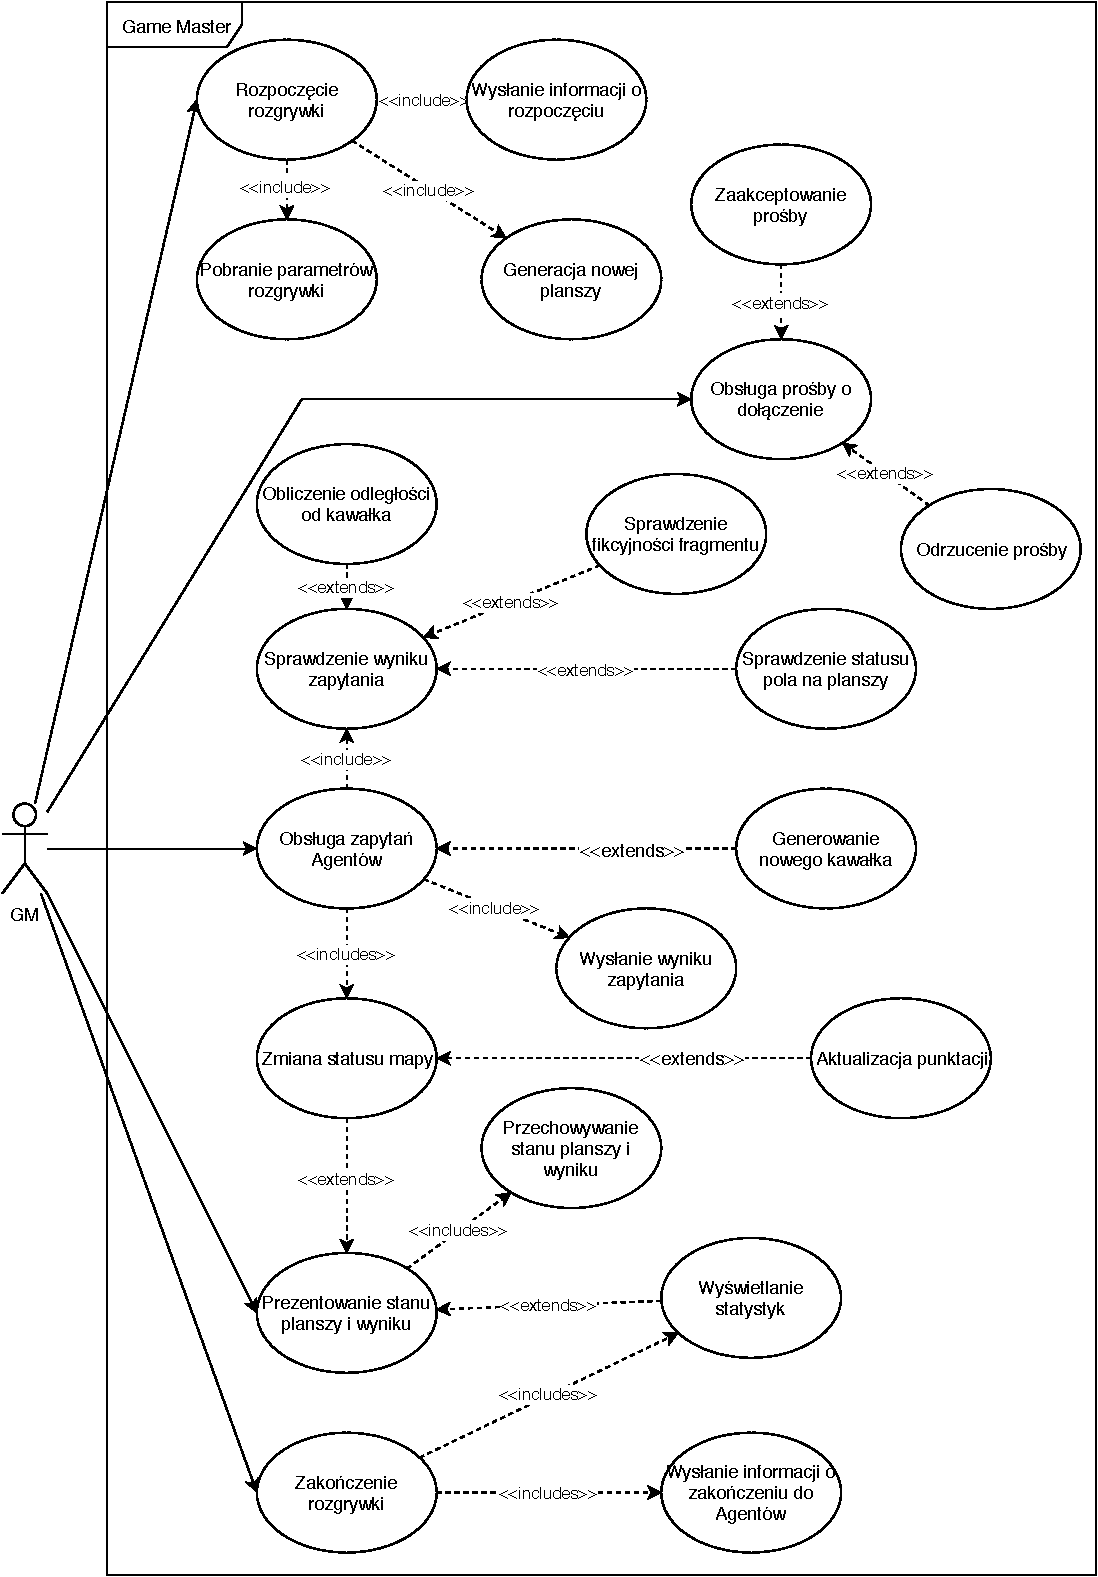
\includegraphics[width=\textwidth]{resources/GM-GM.pdf}

\begin{itemize}
	\item Inicjacja
	\begin{itemize}
		\item GM pobiera parametry rozgrywki z domyslnej konfiguracji, bądź dostarczonej przez użytkownika
		\item Jeśli konfiguracja została podana przez użytkownika Game Master sprawdza czy ilość pól dostępnych na planszy jest większa niż maksymalna ilość graczy, jeśli nie odpytuje użytkownika ponowne wprowadzenie konfiguracji
		\item Nawiązuje połączenie z Serwerem Komunikacyjnym na podstawie danych połączenia zawartych w konfiguracji, w przypadku nieudanej próby połączenia kończy działanie
		\item Generuje nową planszę na podstawie konfiguracji oraz przejście do oczekiwania na dołączenie agentów
	\end{itemize}
	\item Obsługa prosby o dołączenie
	\begin{itemize}
		\item Game Master może odrzucić lub zaakceptować prośbę, w zależnosci od limitu Agentów w drużynie określonej w konfiguracji.
	\end{itemize}
		\item Rozpoczęcie rozgrywki
	\begin{itemize}
		\item Na komendę użytkownika GM rozpoczyna rozgrywkę
		\item Ustala początkowe pozycje każdego z agentów, liderów drużyn i pozycje fragmentów
		\item Wysyła inforamcję o rozpoczęciu do wszystkich agentów, wraz z początkowymi danymi na temat planszy (wielkosć planszy, wielkosć stref punktowych, pozycja startowa Agenta, oraz identyfikatory pozostałych Agentów i ich liderów)
		\item Przechodzi w stan obsługi zapytań agentów
	\end{itemize}
	\item Obsługa zapytań Agentów
	\begin{itemize}
		\item Game Master na podstawie globalnego stanu planszy waliduje zapytanie Agenta i jeśli zapytanie jest nieprawidłowe odsyła informację o błędzie i jego przyczynie
		\item Jesli zapytanie było prawidłowe, GM na podstawie aktualnego stanu mapy generuje odpowiedź dla Agenta i wysyła ją
		\item Akcja agenta może spowodować zmianę stanu planszy, w tym wygenerowanie nowego kawałka jesli akcją było odłożenie fragmentu w polu bramkowym lub zniszczenie go
		\item Akcja agenta może również spowodować zmianę stanu punktacji drużyn, jeśli tak się stało GM powinien sprawdzić czy rozgrywka nie powinna zostać zakończona
	\end{itemize}
	\item Prezentowanie stanu planszy wraz z wynikiem
	\begin{itemize}
		\item Game Master w graficznym interfejsie użytkownika prezentuje aktualny stan planszy, wyniki drużyn oraz meczowe statystyki
		\item Każda akcja zmieniająca stan planszy powoduje aktualizację wyświetlanego widoku
	\end{itemize}
	\item Zakończenie rozgrywki
	\begin{itemize}
		\item Zakończenie rozgrwki może być rezultatem trzech zdarzeń, wygraną którejś z drużyn, zarządaniem zakończenia przez użytkownika oraz utratą połączenia z Serwerem Komunikacyjnym
		\item Po zakończeniu Game Master, o ile to możliwe, wysyła informacje o końcu gry do Agentów i prezentuje statystyki w interfejsie graficznym
	\end{itemize}
\end{itemize}

\end{document}
